\documentclass[11pt,a4paper]{article}
\usepackage{fullpage}
\usepackage[T1]{fontenc} 
\usepackage[utf8]{inputenc}
\usepackage{amsmath}
\usepackage{amssymb}
\usepackage{float}
\usepackage{tabularx}
\usepackage{multirow}
\usepackage{graphicx}
\usepackage{geometry}
\usepackage[table,dvipsnames]{xcolor}
\usepackage[hidelinks]{hyperref}
\usepackage[polish]{babel}
\usepackage{menukeys}
\usepackage{subcaption}

\setlength{\parindent}{0cm}
\setlength{\parskip}{2mm}
\newcolumntype{Y}{>{\centering\arraybackslash}X}
\DeclareMathOperator{\sgn}{sgn}

\begin{document}

\title{Rozpoznawanie człowieka metodami biometrii \\
\Large{
    Projekt 2. --- Rozpoznawanie na~podstawie głosu \\
    Raport
}}
\author{Bartłomiej Dach}
\maketitle

Poniższy dokument stanowi sprawozdanie z~implementacji aplikacji dokonującej rozpoznawania człowieka na~podstawie zarejestrowanych próbek głosu.
W~dokumencie opisano zastosowaną metodę opartą na~współczynnikach mel-cepstralnych oraz~zawarto wyniki działania dla~próbek zarejestrowanych przez~studentów uczęszczających na~zajęcia.

\section{Wstęp}

Ludzki głos jest cechą biometryczną z~pogranicza cech biologicznych i~behawioralnych.
Podczas gdy barwa głosu jest determinowana przez~wrodzone czynniki anatomiczne, ton głosu i~akcent stosowany podczas~wymawiania określonych fraz stanowi cechę nabytą podczas nauki mowy.

Rozpoznawanie człowieka na~podstawie mowy to~prężnie rozwijające~się zagadnienie.
Ze~względu na~rosnącą popularność urządzeń interpretujących frazy wymawiane przez~użytkowników takich, jak~Google Home czy~Amazon Echo, identyfikacja na~podstawie głosu stanowi ważny kierunek rozwoju.

W~ramach projektu zaimplementowano prostą metodę klasyfikacji próbek na~podstawie danego wcześniej zbioru treningowego, używającą współczynników mel-cepstralnych.
Szczegółowy opis metody znajduje~się w~sekcji~\ref{sec:method}.

\section{Opis aplikacji}

Opracowana aplikacja została zaimplementowana w~języku skryptowym~Python w~wersji~3.5.2.
Głównym uzasadnieniem wyboru tego języka był~czas implementacji --- istniejące biblioteki \emph{open source} pozwalają na~szybkie opracowanie algorytmu i~usprawniają proces przetwarzania danych.

Aplikacja ma~postać zbioru skryptów konsolowych --- zdecydowano~się na~rezygnację z~interfejsu graficznego ze~względu na~jego niewielką przydatność w~stosunku do~czasu potrzebnego na~jego opracowanie.
Sposób wywołania skryptów opisany jest w~podsekcji~\ref{sec:manual}.

\subsection{Zastosowane biblioteki}

W~implementacji zastosowano kilka bibliotek \emph{open source}, aby~ominąć konieczność implementacji operacji niezbędnych do~zaimplementowania algorytmu rozpoznawania, takich, jak m.in.~transformata Fouriera.
Pełna lista zastosowanych bibliotek, łącznie z~nazwami licencji, znajduje~się w~tabeli~\ref{tbl:libraries}.

\begin{table}[H]
    \begin{tabularx}{\textwidth}{|r|l|X|l|c|}
        \hline
        Nr & Nazwa & Opis & Licencja & \\
        \hline
        \hline
        1 & \texttt{matplotlib} 3.0.3 & Tworzenie wykresów i~wizualizacji & PSF & \cite{hunter2007} \\
        \hline
        2 & \texttt{numpy} 1.16.2 & Wielowymiarowe tablicowe struktury danych & BSD & \cite{oliphant2006} \\
        \hline
        3 & \texttt{pandas} 0.24.2 & Struktury do~manipulacji i~analizy danych & BSD & \cite{mckinney2010} \\
        \hline
        4 & \texttt{seaborn} 0.9.0 & Rozszerzone wizualizacje danych & BSD & \cite{waskom2018} \\
        \hline
        5 & \texttt{scipy} 1.2.1 & Algorytmy pomocnicze (transformata Fouriera, manipulacja dźwiękiem) & BSD & \cite{jones2001} \\
        \hline
    \end{tabularx}
    \caption{Lista bibliotek użytych w~projekcie}
    \label{tbl:libraries}
\end{table}

\subsection{Instrukcja obsługi}
\label{sec:manual}

W~celu uruchomienia skryptów do~rozpoznawania konieczne jest zainstalowanie interpretera~Python oraz~bibliotek zawartych w~tabeli~\ref{tbl:libraries}.
Aby~zainstalować wymagane biblioteki, należy wywołać polecenie
\begin{verbatim}
$ pip3 install -r requirements.txt
\end{verbatim}
gdzie plik \texttt{requirements.txt} to~plik dołączony do~źródeł aplikacji.

Dla~uproszczenia założono uspójnione nazewnictwo i~format rozpoznawanych próbek.
Próbki powinny być plikami~\texttt{.wav} o~częstotliwości próbkowania 22050~Hz, o~nazwach formatu \texttt{speaker\_XX\_PHRASE\_Y.wav}, gdzie
\begin{itemize}
    \item \texttt{XX} to~numer identyfikacyjny mówcy,
    \item \texttt{PHRASE} to~nazwa identyfikująca frazę, która została zarejestrowana (dla~rozważanego zbioru zarejestrowane zostały cztery frazy: \texttt{biometria}, \texttt{chrzaszcz}, \texttt{poniedzialek} i~\texttt{wycieczka}),
    \item \texttt{Y} to~numer próbki (w~rozważanym zbiorze każda fraza była rejestrowana trzy razy).
\end{itemize}

\subsubsection{Skrypt \texttt{recognize.py}}

Pierwszy ze~skryptów wykonywalnych, o nazwie~\texttt{recognize.py}, dokonuje podstawowego rozpoznawania podanej próbki na~podstawie zbioru próbek treningowych.
Składnia wykonania skryptu~to:
\begin{verbatim}
python3 recognize.py [-h] [-t THRESHOLD]
                     TRAIN_SAMPLE [TRAIN_SAMPLE ...]
                     SAMPLE
\end{verbatim}
gdzie:
\begin{itemize}
    \item opcja \texttt{-h} wyświetla pomoc dot.~wywołania skryptu,
    \item opcja \texttt{-t} (lub \texttt{--threshold}) pozwala na~wyspecyfikowanie progu używanego w~klasyfikacji.
        Domyślnie przyjmowany jest próg $t = 1000$.
        Więcej informacji dot. progu znajduje~się w~podsekcji~\ref{subsec:classification}.
    \item Parametry \texttt{TRAIN\_SAMPLE} to~ścieżki do~próbek używanych do~treningu klasyfikatora.
        Pliki z~próbkami powinny mieć nazwę zawierającą podciąg \texttt{speaker\_XX}, gdzie~\texttt{XX} to~numer~identyfikujący mówcę.
        Wymagane jest podanie co~najmniej jednej próbki.
    \item Parametr \texttt{SAMPLE} to~ścieżka do~pró”ki, która powinna być zaklasyfikowana.
        Możliwe jest podanie tylko jednej próbki.
\end{itemize}
Prawidłowe wywołanie skryptu powoduje wypisanie na~wyjście linii poleceń wyniku klasyfikacji.
W~zależności od~wyniku klasyfikatora próbka może być zakwalifikowana jako~należąca do~jednego z~mówców, lub~jako nieznana próbka.

\subsubsection{Skrypt \texttt{crossvalidator.py}}

Drugi ze~skryptów o~nazwie \texttt{crossvalidator.py} dokonuje kroswalidacji algorytmu klasyfikacji na~podstawie podanego zbioru próbek.
Składnia wykonania skryptu~to:
\begin{verbatim}
python3 crossvalidator.py [-h] SAMPLE_DIR N PHRASE
\end{verbatim}
gdzie:
\begin{itemize}
    \item opcja \texttt{-h} wyświetla pomoc dot.~wywołania skryptu,
    \item parametr \texttt{SAMPLE\_DIR} to~katalog z~próbkami, na~podstawie których wykonywana jest kroswalidacja,
    \item parametr \texttt{N} to~liczba próbek dla~każdego mówcy i~frazy zawartych w~folderze,
    \item parametr \texttt{PHRASE} oznacza frazę, dla~której powinna być wykonana kroswalidacja.
\end{itemize}
Schemat kroswalidacji jest następujący:
\begin{enumerate}
    \item Zbiór próbek dzielony jest na~zbiory: testowy i~treningowy na~$N$ sposobów.
        Dla~$i = 1, \dots, N$ $i$-ty podział ma~$i$-te próbki w~zbiorze treningowym i~wszystkie pozostałe w~zbiorze testowym.
        W~związku z~tym każdy mówca ma~$N - 1$ próbek w~zbiorze treningowym i~jedną w~zbiorze testowym.
    \item Dla~każdego z~podziałów następuje klasyfikacja zbioru testowego (czyli jednej próbki dla~każdego mówcy).
        Wynik klasyfikacji porównywany jest z~docelowym wynikiem, zliczane~są: błędy pierwszej i~drugiej kategorii oraz~pozytywne klasyfikacje.
    \item Skrypt bada również wpływ progu na~jakość klasyfikacji, rozważając wartości progu z~przedziału $[500, 1500]$ z~krokiem 100.
\end{enumerate}
Skrypt tworzy w~katalogu roboczym zbiór wyjściowych plików~\texttt{.csv}, na~podstawie których można oszacować jakość klasyfikacji i~optymalny dobór progu:
\begin{itemize}
    \item Pliki \texttt{confusion\_matrix\_PHRASE\_t=THRESHOLD.csv} zawierają macierze pomyłek dla~wybranej frazy i~wartości progu równej~\texttt{THRESHOLD}.
    \item Plik \texttt{acceptance\_rates\_PHRASE.csv} zawiera liczby: prawidłowych klasyfikacji, fałszywych pozytywów i~fałszywych negatywów dla~danej frazy i~rozważanych wartości progu.
\end{itemize}
Wykresy z~sekcji~\ref{sec:results} zostały wygenerowane na~podstawie tych plików.

\section{Opis metody}
\label{sec:method}

\subsection{Wyznaczanie współczynników mel-cepstralnych}

\subsection{Klasyfikacja nowych próbek}
\label{subsec:classification}

\section{Wyniki eksperymentalne}
\label{sec:results}

\begin{figure}
    \centering
    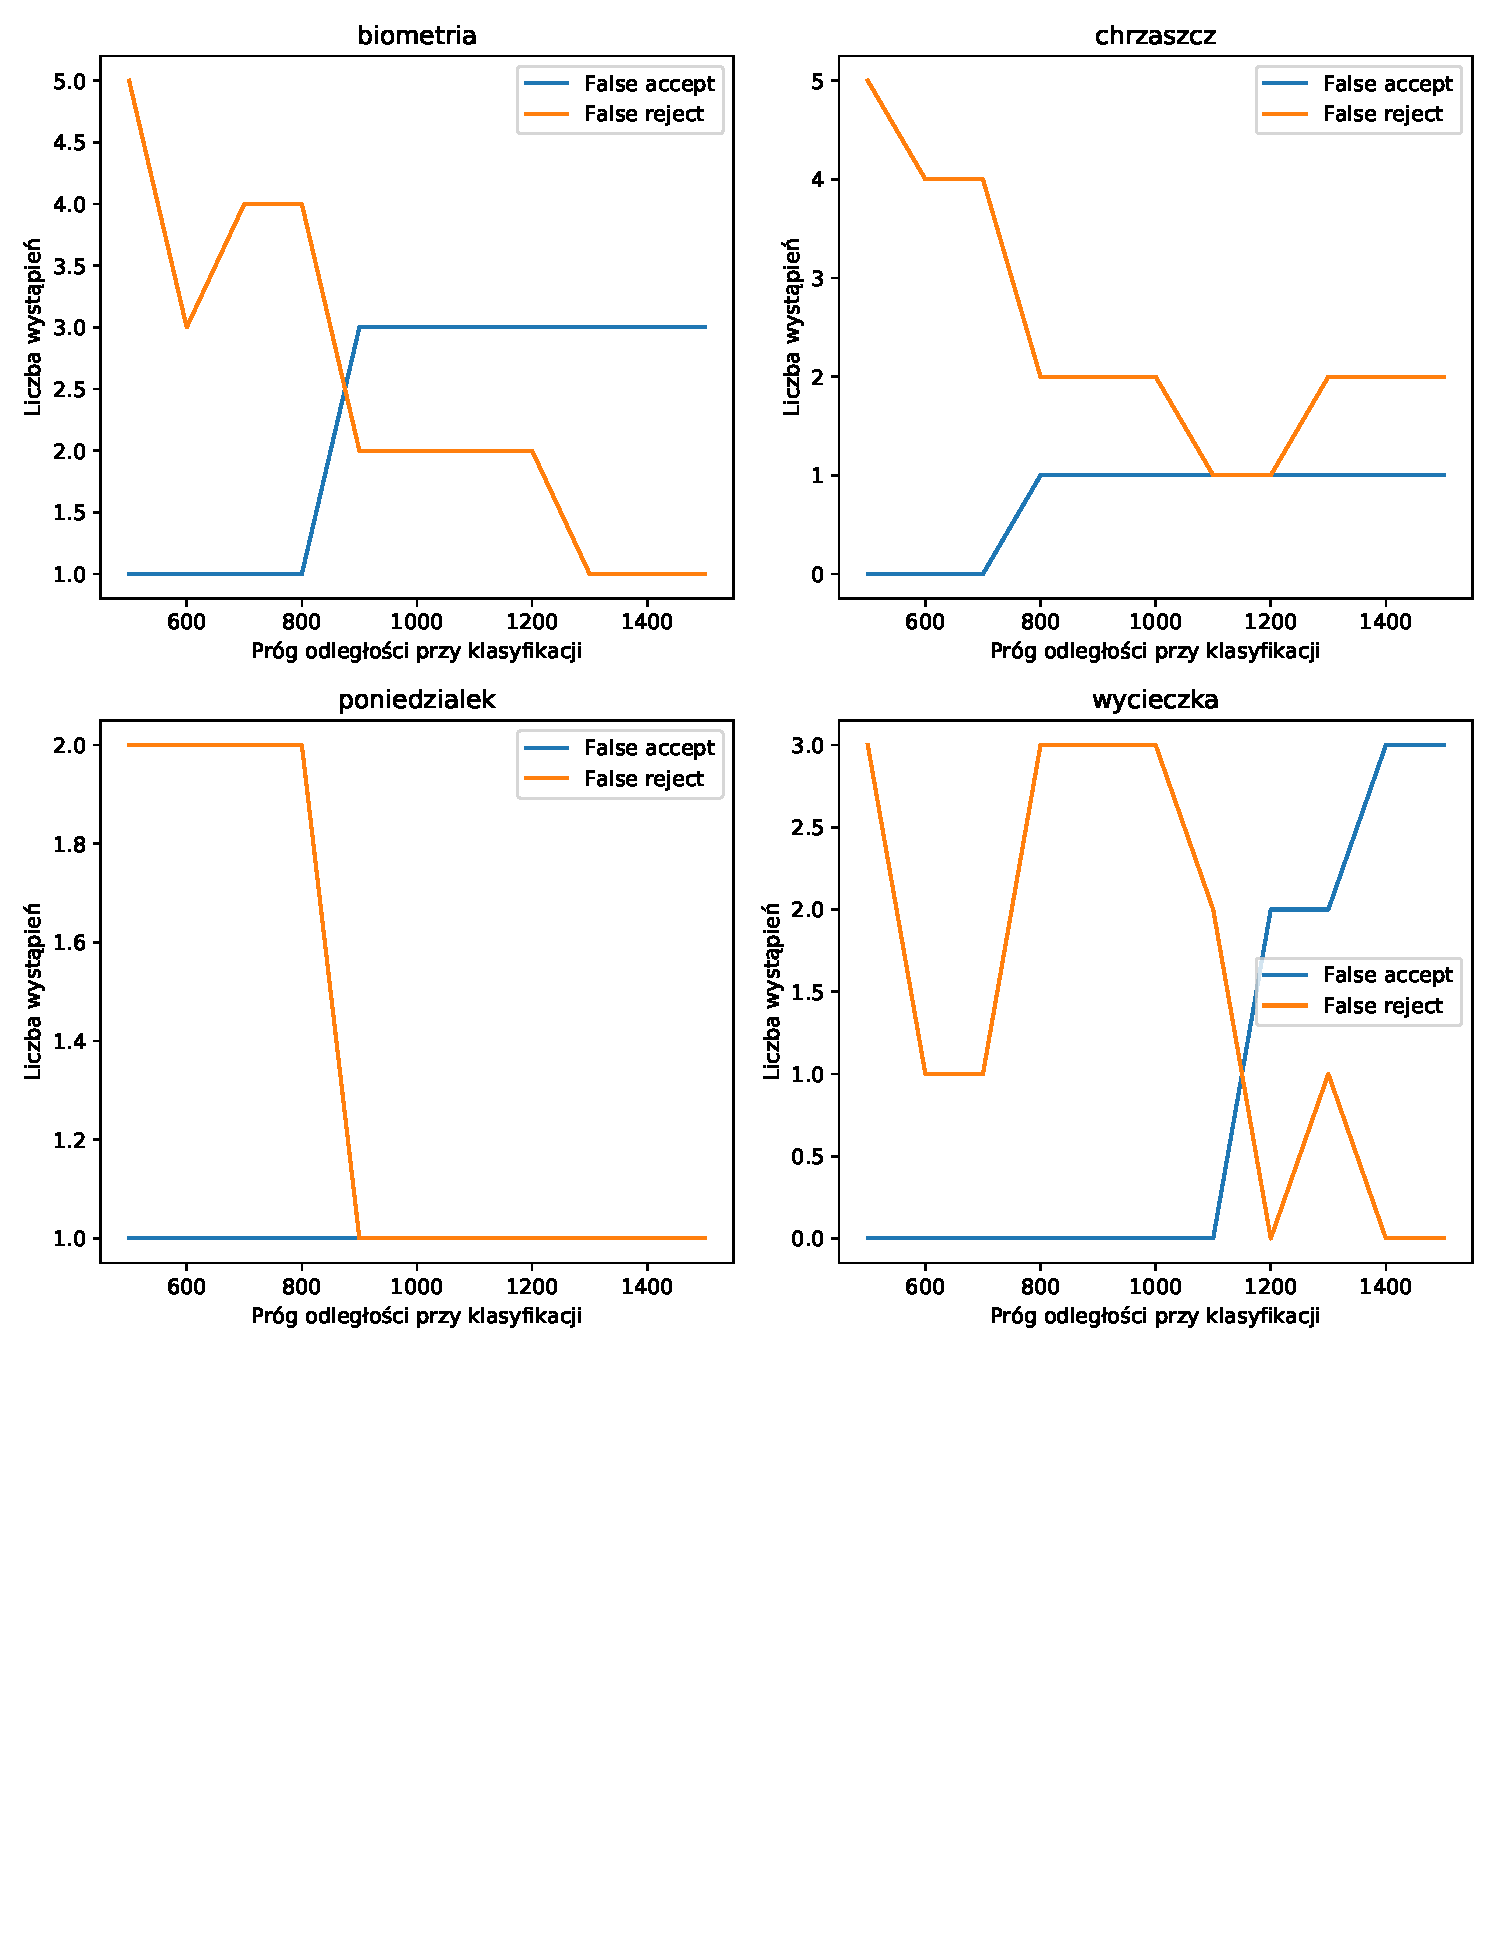
\includegraphics[width=\textwidth]{res/plots/acceptance_rates.pdf}
    \caption{Liczba fałszywych pozytywów (ang.~\emph{false accept}) i~fałszywych odrzuceń (ang.~\emph{false reject}) próbek głosów z~testowanego zbioru w~zależności od~przyjętego progu odległości między~próbkami podczas klasyfikacji.
    Oddzielono wyniki dla~każdej z~czterech rejestrowanych fraz.}
    \label{fig:acceptance-rates}
\end{figure}

\begin{figure}
    \centering
    \begin{subfigure}[t]{0.45\textwidth}
        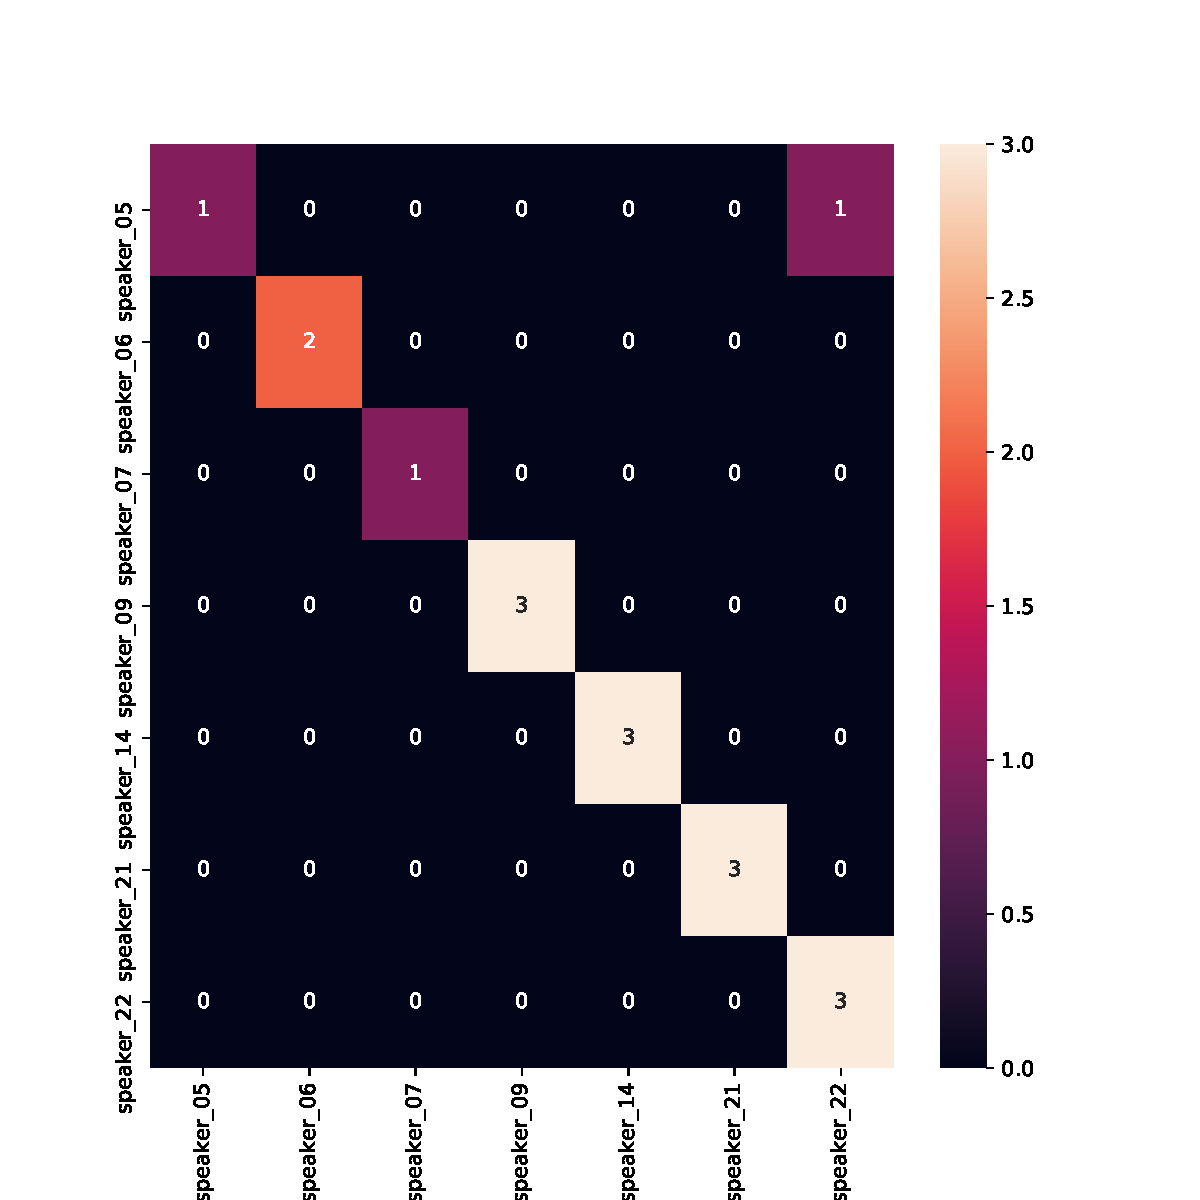
\includegraphics[width=\textwidth]{res/plots/confusion_matrix_biometria.pdf}
        \caption{Macierz pomyłek dla~słowa \emph{biometria} przy~progu~$t = 800$.}
    \end{subfigure}
    \qquad
    \begin{subfigure}[t]{0.45\textwidth}
        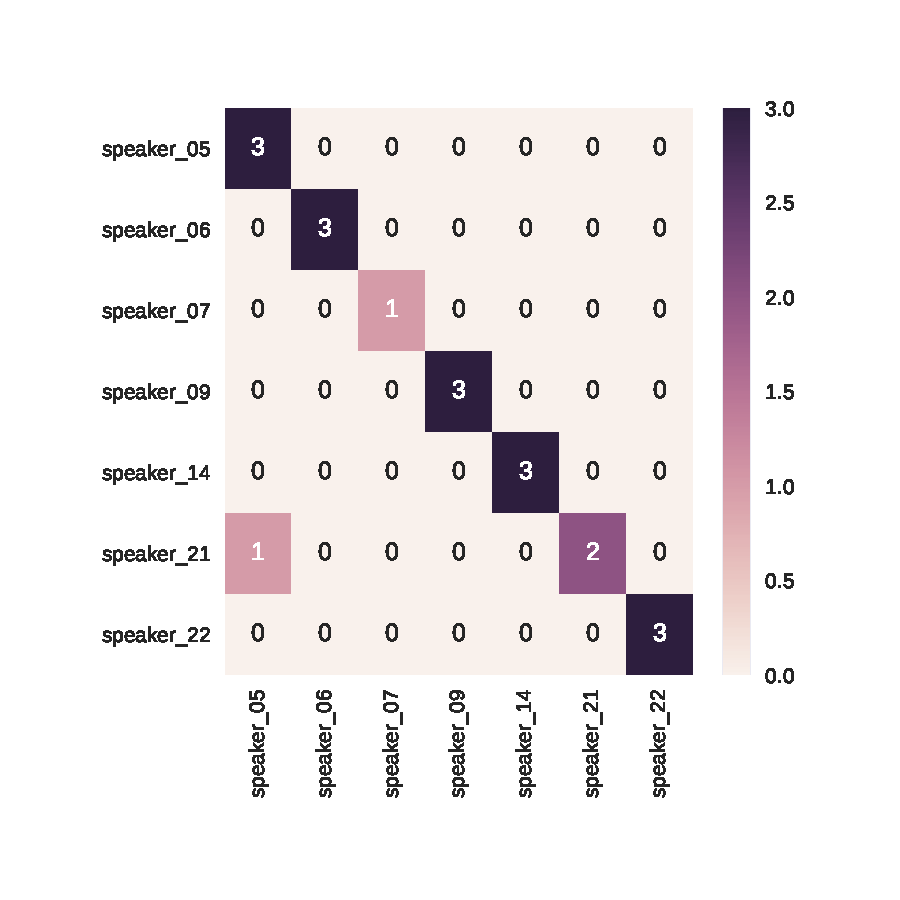
\includegraphics[width=\textwidth]{res/plots/confusion_matrix_chrzaszcz.pdf}
        \caption{Macierz pomyłek dla~słowa \emph{chrząszcz} przy~progu~$t = 800$.}
    \end{subfigure}
    \\
    \begin{subfigure}[t]{0.45\textwidth}
        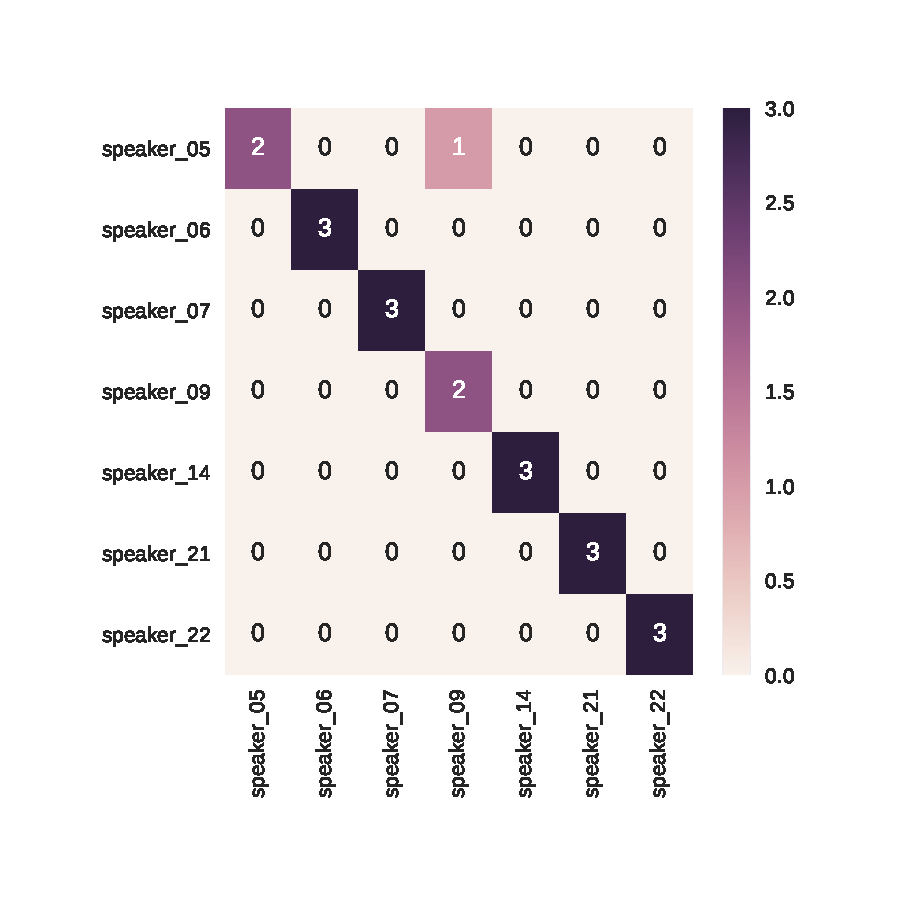
\includegraphics[width=\textwidth]{res/plots/confusion_matrix_poniedzialek.pdf}
        \caption{Macierz pomyłek dla~słowa \emph{poniedziałek} przy~progu~$t = 900$.}
    \end{subfigure}
    \qquad
    \begin{subfigure}[t]{0.45\textwidth}
        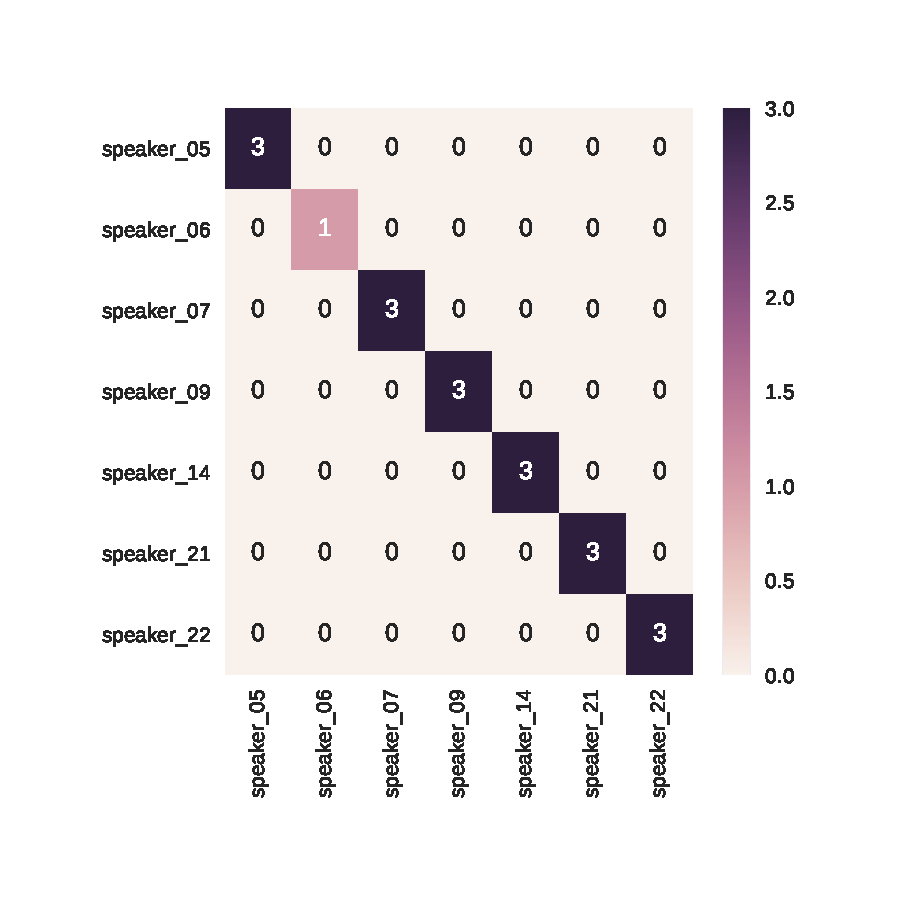
\includegraphics[width=\textwidth]{res/plots/confusion_matrix_wycieczka.pdf}
        \caption{Macierz pomyłek dla~zdania \emph{Jutro pojadę na~wycieczkę, albo~zostanę w~domu} przy~progu~$t = 1100$.}
    \end{subfigure}
    \caption{Macierze pomyłek dla~wartości progu minimalizujących liczbę fałszywych pozytywów i~negatywów dla~poszczególnych zarejestrowanych fraz.}
\end{figure}

\section{Podsumowanie}

\begin{thebibliography}{9}

    \bibitem{hunter2007}
        Hunter, J.D.,
        ,,Matplotlib: A~2D~graphics environment'',
        \emph{Computing In~Science \& Engineering},
        tom~9,
        nr~3,
        s.~90--95,
        2007.

    \bibitem{jones2001}
        Jones, E., Oliphant T.E., Peterson P. i~inni,
        ,,SciPy: Open source scientific tools for~Python''.
        [Online]
        \\
        Dostępne: \url{https://www.scipy.org/}.
        [Dostęp 7 kwietnia 2019]

    \bibitem{mckinney2010}
        McKinney, W.,
        ,,Data Structures for~Statistical Computing in~Python'',
        \emph{Proceedings of~the~9\textsuperscript{th} Python in~Science Conference},
        s.~51--56,
        2010.

    \bibitem{oliphant2006}
        Oliphant, T.E.,
        \emph{A Guide to NumPy},
        Trelgol~Publishing,
        Stany Zjednoczone,
        2006.

    \bibitem{waskom2018}
        Waskom, M. i~inni,
        ,,\texttt{seaborn}: statistical data visualization''.
        [Online]
        \\
        Dostępne: \url{https://seaborn.pydata.org/}.
        [Dostęp 7 kwietnia 2019]

    %\bibitem{slot2008}
        %Ślot K.,
        %\emph{Wybrane zagadnienia biometrii},
        %Wydawnictwa Komunikacji i~Łączności,
        %Warszawa 2008.

\end{thebibliography}

\end{document}
